\documentclass[fontsize=12pt,a4paper,draft]{scrartcl}[2003/01/01]
\usepackage[ngerman]{babel} 
\usepackage[T1]{fontenc}
\usepackage[utf8]{inputenc} 
\usepackage{float}

                           
\usepackage{textcomp}

\title{Robotik Dokumentation - Team Robofreunde n.V.}
\author{Lohr, Schramm, Stumpf, Weber, Wurth}

\date{\today}

%Bilder scalen, wenn größer als Seite
\usepackage[final]{graphicx}
\makeatletter
\def\ScaleIfNeeded{%
	\ifdim\Gin@nat@width>\linewidth
	\linewidth
\else
	\Gin@nat@width
\fi
}
\makeatother


\begin{document}
Es handelt sich hier nur um einen Vorschlag für die Struktur des Dokuments. Das Ding erhebt keinen Anspruch auf Vollständigkeit, sondern ist das Ergebnis von maximal 15 Minuten \glqq Fuck, wir müssen den Shit fertig machen, ich fang mal an lol\grqq. Bevor wir dann wirklich anfangen aufzuteilen, wer was schreibt (abseits der offensichtlichen Stellen), sollten wir die Struktur des Dokuments \textbf{zusammen} durchgehen und finalisieren. Btw, ich hab keinen Plan von Latex, sollte ich also gegen irgendwelche Konventionen verstoßen haben würde es mich nicht wundern... Hoffe aber es passt einigermaßen. Manu

\maketitle
\tableofcontents

\section{Einleitung}
\textit{Ein paar einleitende Sätze. (Was ist Robocup und so...)}
\section{Anforderungen}
\textit{Was waren die allgemeinen Anforderungen?}
\section{Zeitplan}
\textit{Was wurde wann gemacht?}
\section{Framework}
\textit{Ein paar einleitende Sätze.}
\subsection{Entscheidung für Magma}
\textit{Warum Magma?}
\subsection{Überblick Magma}
\textit{Alles, was wir so über das Framework rausgefunden haben und erwähnenswert ist.}

\section{KI-Konzept}
Für die KI wurde ein Konzept entwickelt, dass sich einfach in die bereits existierende Architektur des verwendeten Frameworks integrieren ließ. Ziel war es, eine möglichst flexible und gleichzeitig einfache Architektur zu entwerfen. Das Ergebnis ist eine Schichten-Architektur, deren Teilkomponenten einfach verändert oder ausgetauscht werden können. Nebeneffekte auf andere Module sind durch die Architektur weitgehend ausgeschlossen. So war es beispielsweise Problemlos möglich, verschiedene Herangehensweisen für die Implementierung von Rollen in das Gesamtsystem zu integrieren. Verschiedene Teammitglieder konnten also ihre selbst entwickelten Rollen schnell und einfach in das Gesamtsystem integrieren, ohne andere Komponenten anpassen zu müssen.

\subsection{Anforderungen}
Das gewählte Framework und die Tatsache, dass eine Steuerung für eigenständige Roboter entwickelt werden musste, stellt einige Anforderungen an die zu entwickelnde künstliche Intelligenz.\\
\\
Jeder Roboter ist als unabhängiges Individuum zu verstehen. Das hat die direkte Folge, dass Entscheidungen nicht von einer übergeordneten Instanz getroffen werden können; Jeder Roboter muss aufgrund der ihm zur Verfügung stehenden Informationen seine eigenen Entscheidungen treffen. Das Fehlen einer zentralen Komponente erschwert es erheblich, ein aufeinander abgestimmtes Team-Spiel zu entwickeln. Dennoch gibt es für dieses Problem gute Ansätze. Die Anforderung, die sich zusammenfassend daraus ableiten lässt, ist die Notwendigkeit einer dezentralen Lösung für die KI.\\
\\
Eine weitere Anforderung ergibt sich aus der Wahl des Frameworks. Das Framework arbeitet weitgehend mit Polling, also einem kontinuierlichen Abfragen der nächsten Aktion. Es ist daher naheliegend, auch für die hier zu entwickelnde KI einen Ansatz mit Polling zu zu verfolgen.\\
\\
Neben den mehr oder weniger durch die äußeren Umstände vorgegebenen Anforderungen haben wir noch weitere zwei Anforderungen definiert. Roboter sollen ihre Rolle dynamisch wechseln, außerdem soll es zusätzlich die Möglichkeit geben, die aktuell verfolgte Spiel-Strategie nach Bedarf zu ändern.

\subsection{Komponenten}
Das KI-Grundkonzept besteht aus insgesamt 4 Schichten. Jede Schicht kennt ausschließlich die darunterliegende Schicht. Die unterste Ebene definiert Grundlegende Bewegungen eines Roboters. Direkt darüber befinden sich Rollen. Rollen sind zum Beispiel \glqq Stürmer\grqq oder \glqq Torwart\grqq, aber auch Spezialrollen wie \glqq Anstoß\grqq oder \glqq Freistoß\grqq. Über den Rollen befindet sich die Strategie-Ebene. Auf höchster Ebene befindet sich der Strategie-Entscheider.

\subsubsection{Elementare Bewegungen}
Elementare Bewegungen sind die Grundlage für alle höheren Schichten. Sie sind die unmittelbare Voraussetzung die darüber liegenden Rollen, weil sie von diesen direkt benutzt werden. Elementare Bewegungen sind zum Beispiel: \glqq Laufen\grqq, \glqq Aufstehen\grqq, \glqq Schießen\grqq, oder \glqq Dribbeln\grqq. Abgesehen vom \glqq Dribbeln\grqq waren alle Bewegungen bereits mehr oder weniger funktionsfähig im Framework vorhanden. Dennoch musste an einigen Stellen optimiert und angepasst werden, siehe Kapitel \ref{Mechanik}.

\subsubsection{Rollen}
Rollen definieren das Grundlegende Verhalten eines Roboters. Ein Verteidiger verfolgt eine andere Spielweise als ein Torwart. Alle unsere Rollen sind Statemachines. Eine wichtige Frage ist, wo und wie die KI für Standard-Situationen wie zum Beispiel den \glqq Anstoß\grqq in der Architektur verankert werden soll. Eine naheliegende Lösung ist die Definition von Spezialrollen, die genau diese Standard-Situationen behandeln. Die Alternative wäre eine Erweiterung aller Standard-Rollen um die Algorithmik der Standard-Situationen. Einen wirklichen Mehrwert hat man dadurch allerdings nicht, denn der Algorithmus um einen Anstoß zu machen benötigt keine Routinen eines Stürmers. Umgekehrt gilt das Selbe. Die Entscheidung fiel also auf die Definition von Spezialrollen, die genau diese Standard-Situationen umsetzen. Ein Spieler, der normalerweise zum Beispiel Stürmer ist, wechselt bei Bedarf einfach seine Rolle in \glqq Anstoß\grqq und im Anschluss wieder zurück.

\begin{figure}[H]
	\centering
	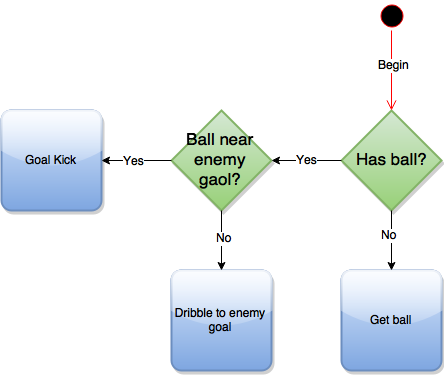
\includegraphics[width=0.7\textwidth]{Grafiken/KI/simple_Player}
	\caption[Beispiel Rolle: Keeper]{Beispiel Rolle: Keeper}
\end{figure}


\subsubsection{Strategien}
Rollen sollen nicht selbst entscheiden, ob und in welche andere Rolle gewechselt wird. Das widerspräche der Schichtenarchitektur. Deshalb wurde die darüber liegende Strategieschicht eingeführt. Die Aufgabe dieser Schicht ist es, Rollen dynamisch zuzuordnen. Daher ist die Bezeichnung \glqq Strategie\grqq auch treffend; Eine Strategie steuert unter Anderem die Gesamtaufstellung des Teams. Damit lässt sich die allgemeine Spielweise des gesamten Teams steuern, mehr Verteidiger bedeutet eine defensive, mehr Angreifer eine aggressive Strategie. Eine Strategie benötigt einen Pool an Rollen, die sie \glqq verteilen\grqq darf. Dieser Pool definiert die grundlegende Spielweise eines Teams. Aufgabe jeder Strategie ist es dann, Rollen dynamisch nach Bedarf zu verteilen. Darunter fällt auch die Vergabe der Spezialrollen.

\subsubsection{Strategie-Entscheider}
In der Strategieebene können verschiedene Strategien für verschiedene Gesamtaufstellungen des Teams definiert werden. Im Laufe eines Spiels kann es sinnvoll sein, die Aufstellung an die Gegebenheiten und Anforderungen an das Spiel anzupassen. Dafür Wurde auf höchster Ebene ein Entscheidungsmechanismus etabliert. Die Aufgabe dieser Schicht ist es, je nach Bedarf eine passende Strategie auszuwählen. Dafür gibt es verschiedene Ansätze, zum Beispiel könnte eine passende Strategie je nach aktuellem Spielstand ausgesucht werden. Beispiel: 
\begin{itemize}
\item Mannschaft liegt vorne: Defensive Strategie
\item Unentschieden: Aggresive Strategie
\item Mannschaft liegt hinten: Aggressive Strategie
\item Mannschaft liegt hinten und Zeit läuft bald aus: Risiko Strategie
\end{itemize}
\subsection{Gesamtübersicht}

\section{Elementare Bewegungen}
\textit{Hier kommt der Stuff rein, der angepasst werden musste \dots
(Laufen, Schießen und son shiat). (Subsections machen!)}

\section{Rollen}

\subsection{Standard Rollen}

\subsubsection{Torwart}
\subsubsection{Verteidiger}
\subsubsection{Mittelfeld}
\subsubsection{Stürmer}

\subsection{Spezielle Rollen}
\textit{Bastus}
\section{Grafisches Debugging}
\textit{Felix do your thing}

\section{Strategien}

\section{Strategie-Entscheider}

\section{Zusammenfassung und Ausblick}
\textit{Ergebnisse und Vermächtnis...}

\section{Verzeichnisse}
\listoffigures
\end{document}